
\let\negmedspace\undefined
\let\negthickspace\undefined
\documentclass[journal,12pt,twocolumn]{IEEEtran}
\usepackage{cite}
\usepackage{amsmath,amssymb,amsfonts,amsthm}
\usepackage{graphicx}
\usepackage{textcomp}
\usepackage{xcolor}
\usepackage{txfonts}
\usepackage{listings}
\usepackage{enumitem}
\usepackage{mathtools}
\usepackage{gensymb}
\usepackage[breaklinks=true]{hyperref}
\usepackage{tkz-euclide} % loads  TikZ and tkz-base
\usepackage{listings}
\usepackage{gvv}
\usepackage{booktabs}

%
%\usepackage{setspace}
%\usepackage{gensymb}
%\doublespacing
%\singlespacing

%\usepackage{graphicx}
%\usepackage{amssymb}
%\usepackage{relsize}
%\usepackage[cmex10]{amsmath}
%\usepackage{amsthm}
%\interdisplaylinepenalty=2500
%\savesymbol{iint}
%\usepackage{txfonts}
%\restoresymbol{TXF}{iint}
%\usepackage{wasysym}
%\usepackage{amsthm}
%\usepackage{iithtlc}
%\usepackage{mathrsfs}
%\usepackage{txfonts}
%\usepackage{stfloats}
%\usepackage{bm}
%\usepackage{cite}
%\usepackage{cases}
%\usepackage{subfig}
%\usepackage{xtab}
%\usepackage{longtable}
%\usepackage{multirow}

%\usepackage{algpseudocode}
%\usepackage{enumitem}
%\usepackage{mathtools}
%\usepackage{tikz}
%\usepackage{circuitikz}
%\usepackage{verbatim}
%\usepackage{tfrupee}
%\usepackage{stmaryrd}
%\usetkzobj{all}
%    \usepackage{color}                                            %%
%    \usepackage{array}                                            %%
%    \usepackage{longtable}                                        %%
%    \usepackage{calc}                                             %%
%    \usepackage{multirow}                                         %%
%    \usepackage{hhline}                                           %%
%    \usepackage{ifthen}                                           %%
  %optionally (for landscape tables embedded in another document): %%
%    \usepackage{lscape}     
%\usepackage{multicol}
%\usepackage{chngcntr}
%\usepackage{enumerate}

%\usepackage{wasysym}
%\documentclass[conference]{IEEEtran}
%\IEEEoverridecommandlockouts
% The preceding line is only needed to identify funding in the first footnote. If that is unneeded, please comment it out.

\newtheorem{theorem}{Theorem}[section]
\newtheorem{problem}{Problem}
\newtheorem{proposition}{Proposition}[section]
\newtheorem{lemma}{Lemma}[section]
\newtheorem{corollary}[theorem]{Corollary}
\newtheorem{example}{Example}[section]
\newtheorem{definition}[problem]{Definition}
%\newtheorem{thm}{Theorem}[section] 
%\newtheorem{defn}[thm]{Definition}
%\newtheorem{algorithm}{Algorithm}[section]
%\newtheorem{cor}{Corollary}
\newcommand{\BEQA}{\begin{eqnarray}}
\newcommand{\EEQA}{\end{eqnarray}}
\newcommand{\define}{\stackrel{\triangle}{=}}
\theoremstyle{remark}
\newtheorem{rem}{Remark}

%\bibliographystyle{ieeetr}
\begin{document}
%

\bibliographystyle{IEEEtran}


\vspace{3cm}

\title{
%	\logo{
Discrete Assignment 

\large{EE:1205 Signals and Systems}

Indian Institute of Technology, Hyderabad
%	}
}
\author{Abhey Garg

EE23BTECH11202
}	


% make the title area
\maketitle

\newpage

%\tableofcontents

\bigskip

\renewcommand{\thefigure}{\theenumi}
\renewcommand{\thetable}{\arabic{table}}
%\renewcommand{\theequation}{\theenumi}

\section{Question 10.5.2.13}
How many 3 digit numbers are divisible by 7?
\section{Solution}

\begin{table}[ht]
\centering
\setlength{\extrarowheight}{8pt}
\caption{Input Parameters}
\begin{tabular}{|c|l|l|} 
\hline
\textbf{Parameter} & \textbf{Used to denote} & \textbf{Values} \\
\hline
$x$\brak{0}  & First Term & \multicolumn{1}{|p{1.5cm}|}{\centering $x\brak{0} = 105$ }\\
\hline
$d$ & Common difference of A.P & \multicolumn{1}{|p{1.5cm}|}{\centering $d = 7 $ } \\
\hline

\end{tabular}
 \vspace{4mm}
 \label{tab:table0}
\end{table}


Three digit numbers which are divisible by 7 are \(105, 112, 119, \ldots, 994\), which form an arithmetic progression (A.P). 
The number of terms in the AP x\brak{n} is given by: 
\begin{align}  \label{eq:eq12}
    \frac{x\brak{n} - x\brak{0}}{d}  + 1
\end{align}
\begin{align}
    &X_i(z) = \frac{x_i\brak{0}}{1 - z^{-1}} + d_i\frac{z^{-1}}{\brak{1-z^{-1}}^2} \text{ , for i=1,2} \label{eq:eq3}
\end{align}
\quad{ROC : $\abs{z} > 1$ as it is an AP}   
\begin{align}
x_{1}\brak{n} &= \brak{105 + \brak{n}7}u\brak{n}
\end{align}
Using the values in \tabref{tab:table0} :
\begin{align}
    k_1 = \frac{994 - 105}{7} + 1 = 128
\end{align}
Using the values in \tabref{tab:table0} :
\begin{align}
 X_1\brak{z} = \frac{105 - z^{-1}}{\brak{1-z^{-1}}^2}
\end{align}
ROC is $\abs{z} > 1$

\begin{figure}[!ht]
\centering
\begin{center}
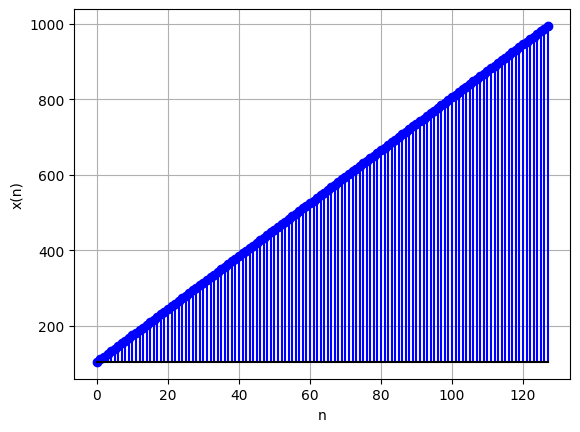
\includegraphics[width=\columnwidth]{figs/Fig1}
\caption{Plot of $x\brak{n}$}
\end{center}
\end{figure}
	
\end{document}